Automated model verification is only useful to us as far as the generated counterexamples are comprehensible. Without comprehensible counterexamples, the negative verification results provide very little or no insight into the source of the error. The fairness constraint used in this project introduces an issue into the counterexamples. Because the fairness property is a prerequisite for every other property, the execution error trails must end in a valid end state. This means that regardless of where an error actually occurs, the trail will always continue until the valid end state is reached. Therefore, at first glance, there is a chance that many error trails will look very similar (or even identical) to each other. The tool explained in this section aims to assist the user in both identifying the moment(s) of failure for each counterexample and also uniquely identify each error trail.

The error visualizer is a mechanism to visualize both the workflow and the CWP as they evolve along the error trace. This allows the user to identify the moment the CWP was violated and examine the history preceding the error. A set of annotated images are generated for both the workflow and CWP. Each annotated image corresponds to a single step of execution during the verification process. A step is characterized by the execution of an element in the BPMN. The execution of each element initiates another step in the counterexample. \figref{fig:ErrorVisualizationRoadmap} shows the high-level process of generating the error visualization output. 

\begin{figure*}[t]
  \begin{center}
    \begin{tabular}{c}
        \frame{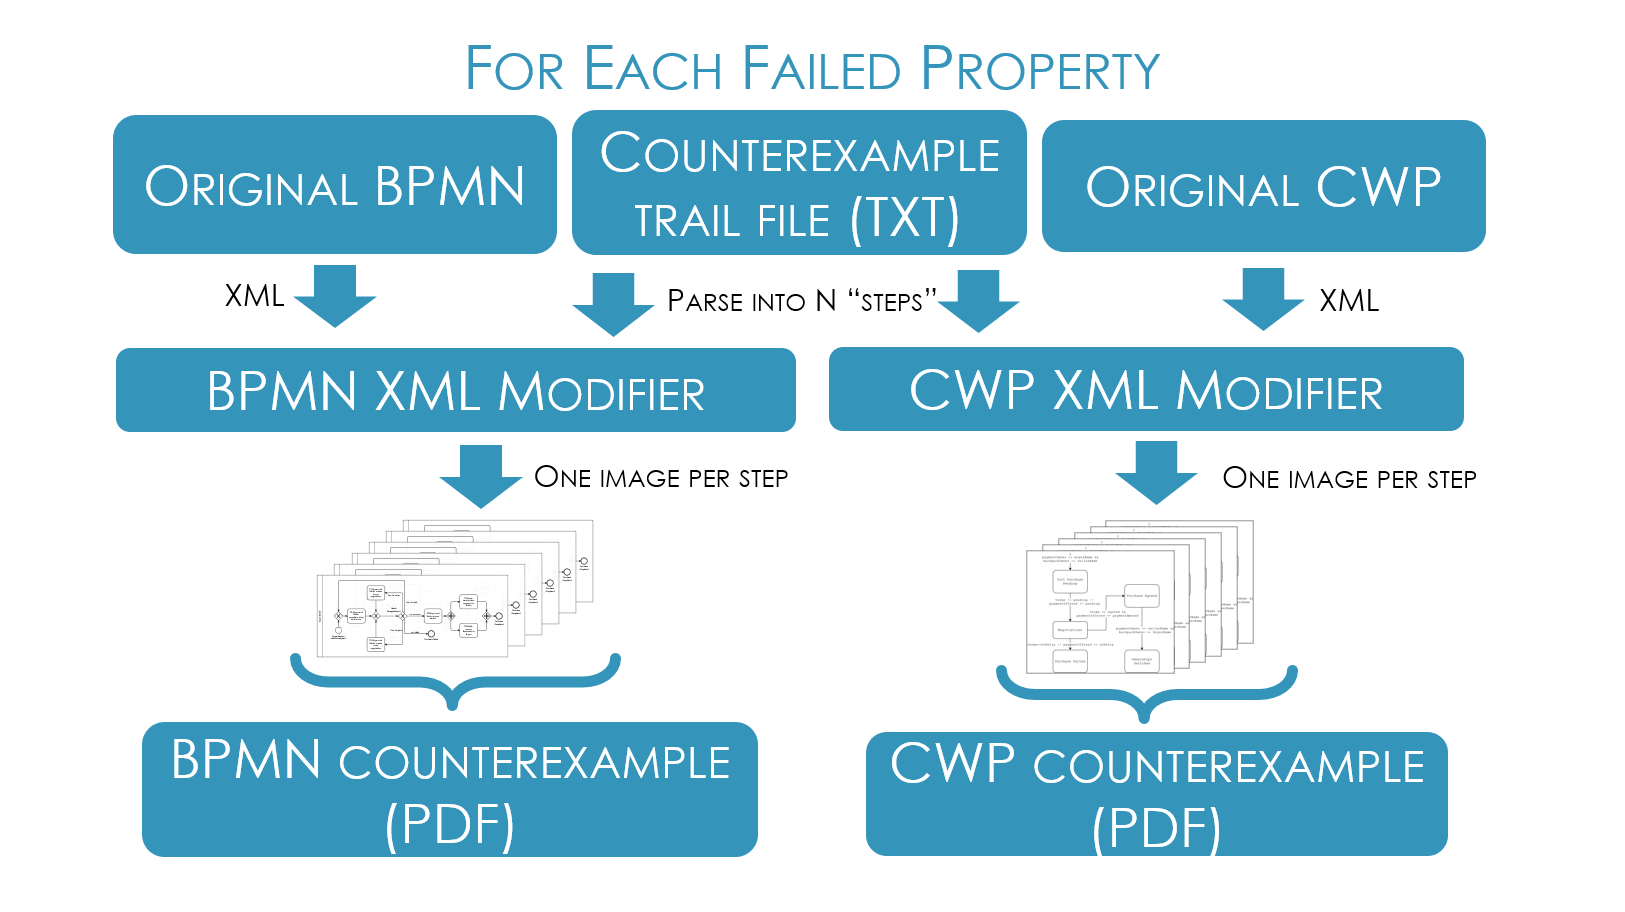
\includegraphics[width=\textwidth]{../figs/Other/ErrorVisualizationRoadmapWhiteBG.png}}
    \end{tabular}
  \end{center}
\caption{Error Visualization Generation Pipeline}
\label{fig:ErrorVisualizationRoadmap}
\end{figure*}


An example annotated BPMN image for step 1 is shown in \figref{fig:ErrorVisualizationBPMN} and the corresponding CWP is shown in \figref{fig:ErrorVisualizationCWP}. Step 1 is the initial step where the start event is executed and the token moves toward the first XOR gateway.

\begin{figure*}[t]
  \begin{center}
    \begin{tabular}{c}
        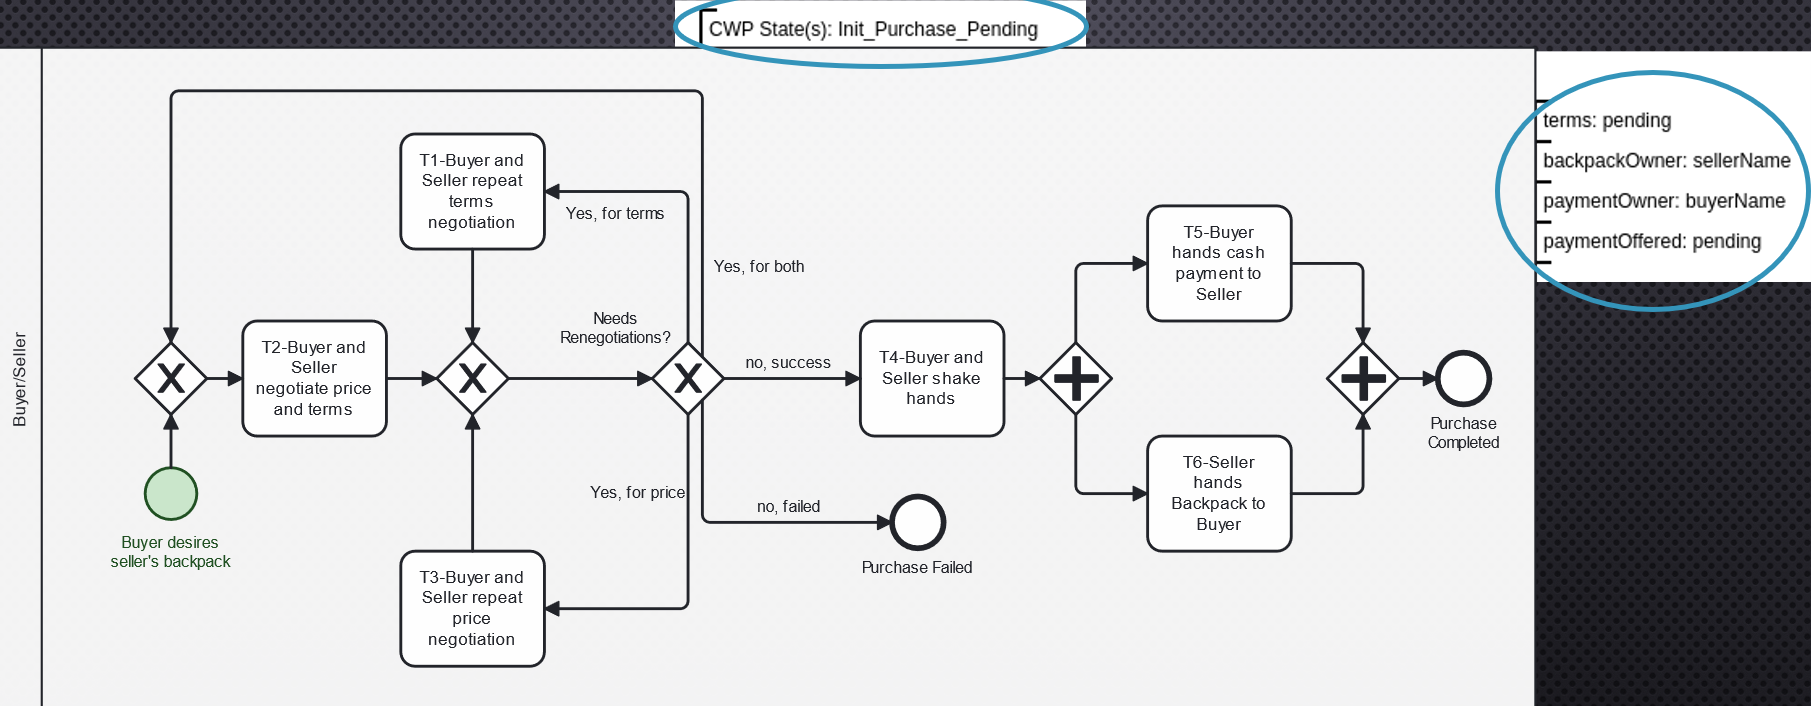
\includegraphics[width=\textwidth]{../figs/Other/ErrorVisualizationBPMN.png}
    \end{tabular}
  \end{center}
\caption{Annotated BPMN for the first step of an error in Face2Face}
\label{fig:ErrorVisualizationBPMN}
\end{figure*}


\begin{figure*}[t]
  \begin{center}
    \begin{tabular}{c}
        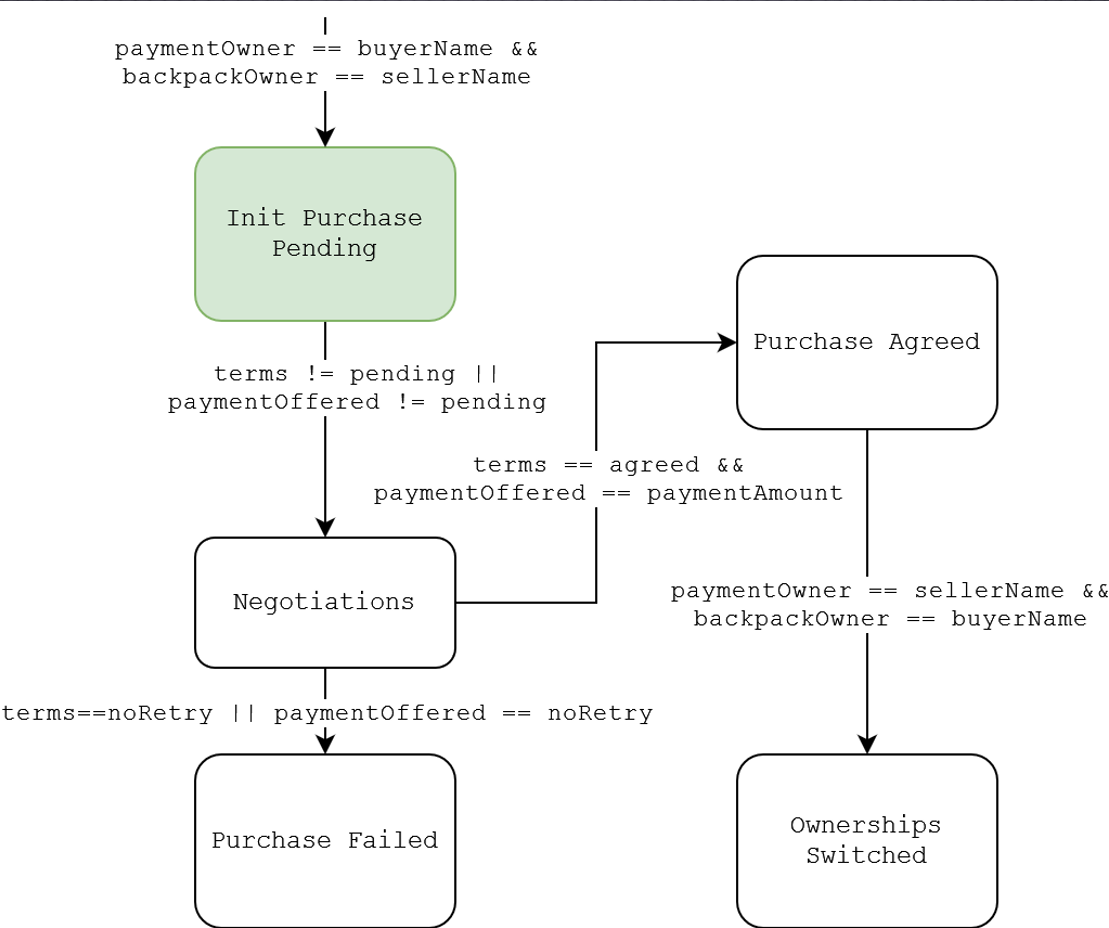
\includegraphics[width=\textwidth]{../figs/Other/ErrorVisualizationCWP.png}
    \end{tabular}
  \end{center}
\caption{Annotated CWP for the first step of an error in Face2Face}
\label{fig:ErrorVisualizationCWP}
\end{figure*}

Aside from the path of execution, there are several notable annotations, particularly on the BPMN. First, at the top of the BPMN workflow, there is a list of the state(s) in which the BPMN currently resides. This is important to pay attention to because it will show precisely when a property is violated. For example, if any "mutex" property is violated, there will eventually be a step in execution that lists multiple states at the top of the image. This moment is the moment of failure. Additionally, if the "alwaysInAState" property fails, there will eventually be a step in which no states are listed.

Next, in the top right corner of the BPMN workflow, each of the object state variables are listed, along with their current values. This information can help a user find subtle errors involving CWP edge labels, BPMN behavior models, and more. Each variable is highlighted if its value is changed after the current BPMN step is finished.

To assist with distinguishing similar or identical trails, an annotation is included in the top center that indicates possible moments of interest for the specific property in question. This feature indicates moments where the underlying LTL property takes a step (meaning that something interesting happened in regards to the logical expressions referenced in the property.)

Finally, the CWP image is annotated by coloring the current state(s). If the BPMN only resides in one state, it is colored green. If the BPMN resides in multiple states simultaneously, they will be colored red. Additionally, if on the previous step, the BPMN resided in a state from which there is not a transition to the current state, the current state will be colored red.

It is important to note that the visualizer shows the BPMN first taking a step, followed by the CWP updating. Therefore, the annotated CWP image associated with step $n$ indicates that the corresponding BPMN resides in the colored state(s) after it has taken its $n$th step. The state annotation and the object state variables annotation on the BPMN image also represent the object state \emph{after} the BPMN takes its step.

The counterexample visualizer currently has limitations in regards to existential properties. An existential property is one that is proven by finding a witness - a trail that shows some state exists in the model. A witness is manifest as an error in SPIN, but the absence of a witness means the property failed to verify. In this case, the counterexample visualizer has nothing to report, except that a witness was not found. More informative reporting of these cases is a difficult question that is left for future work.
